\subsection{Interlude 2: What's up witht the Early Effect?}
Very, very important thing to start with: it's named after James Early, and is not related to being early, late or anything time related. I wanted to mention it first because to this day I unconsciously picture it as something happening before something else. 
The lecture notes state: "When deriving the I-V (Current-Voltage) characteristics of nFETs in the previous chapter, we assumed that the current is constant when working in saturation ($V_{ds} > 4U_T$). It so happens that this assumption is not sufficient, especially with short length MOSFETs, for which the drain voltage can modulate the channel current, even in saturation." So what is exactly happening here?  
Let's start by reminding ourselves the (nFET) relationship and the theoretical graph linking drain current $I_{ds}$ to drain to source voltage $V_{ds}$ for fixed $V_{gs}$:

\begin{equation}
I_{ds} = I_{n0} e^{\frac{\kappa_{n}V_g}{U_T}}(e^\frac{-V_s}{U_T} - e^\frac{-V_d}{U_T})
\end{equation}

We also should look at the graphical relationship this relation implies:

\begin{figure}[H]
    \centering
    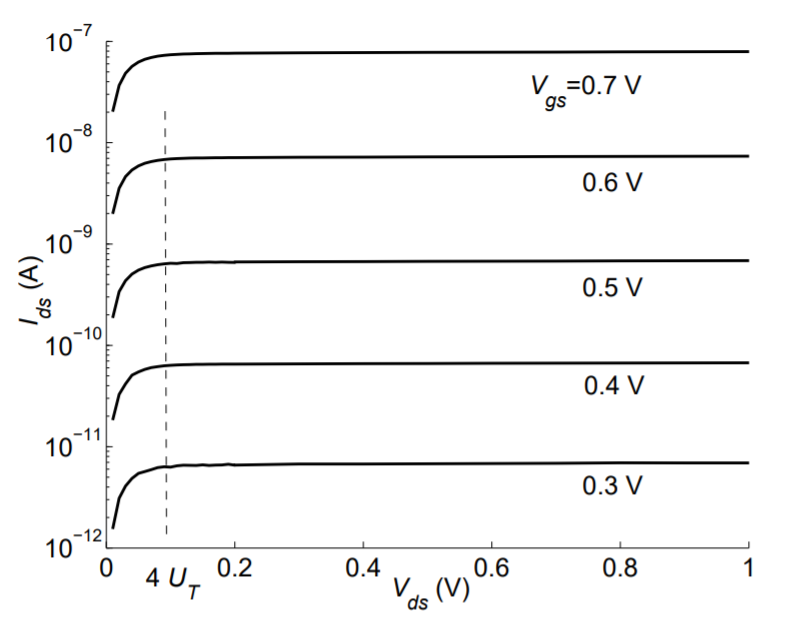
\includegraphics[width=0.95\linewidth]{../../Figures/Vds_Vs_Ids_No_Early_Effect.PNG}
    \caption{Relationship between $V_{ds}$ and $I_{ds}$ for fixed $V_{gs}$. Determines the voltage at which we switch from Ohmic to Saturation region. Adapted from Lecture Notes.}
    \label{fig:basalandcerebellum}
\end{figure}

One should notice in the equation and that $I_{ds}$ has an almost insignificant dependence on $V_{ds}$, because of the exponential term, where the term in parenthesis just vanishes to $V_{s}$ as $V_{d}$ (and thus $V_{ds}$) increases. We consider this to start being true when $V_{ds} > 4$U_T$, where we go from the "Ohmic" Region to the "Saturation region". This is clearly apparent in the above figure, where changing $V_{ds}$ does not affect $I_{ds}$ past the 4$U_T$ threshold - thus yielding a constant relationship between $V_{ds}$ and $I_{ds}$ past the threshold (again, taking $V_{gs}$ as fixed). 

Now surprise surprise, this model is not correct in practice. This is called the Early effect, and basically introduces the practical problem of slightly rising $I_{ds}$ when increasing $V_{ds}$, even past the the saturation threshold. This rate of change is critically impacted by the geometry of the transistor, mainly its W/L ratio. Effectively, when increasing $V_d$, the \emph{effective length $L_{eff}$} of the transistor decreases. This is because the pinchoff region extends further along the channel away from the drain (see figure below). This has a particularly important impact when we are dealing with short transistors, as the shift in pinchoff is, relatively to the channel length, more important. 

\begin{figure}[H]
    \centering
    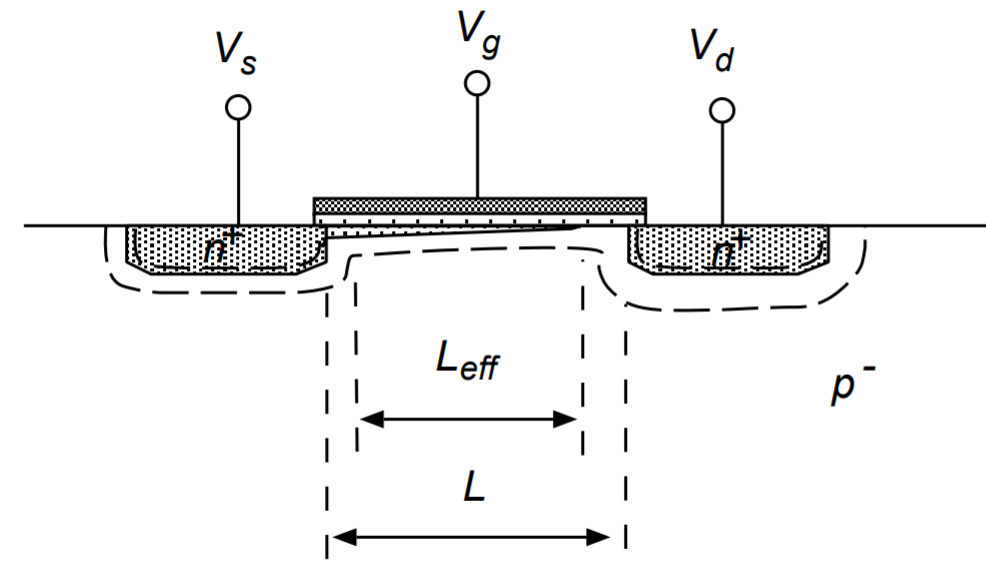
\includegraphics[width=0.95\linewidth]{../../Figures/Early_Effect_Pinchoff_Region.PNG}
    \caption{The effective channel length $L_{eff}$ of a transistor operating in the above-threshold saturation region decreases with increasing Vd because the pinchoff point moves into the channel, away from the drain. The effective channel length can be described by the transistor length minus the length of the pinchoff region in the channel. Adapted from Lecture Notes.}
    \label{fig:basalandcerebellum}
\end{figure}

Ok great. So what do we do with this information? Well now we need to find a way to quantify this effect and include it in the previous equation to have a more accurate model. For this, we need to use the \emph{Early Voltage} and the following relations: 

\begin{figure}[H]
    \centering
    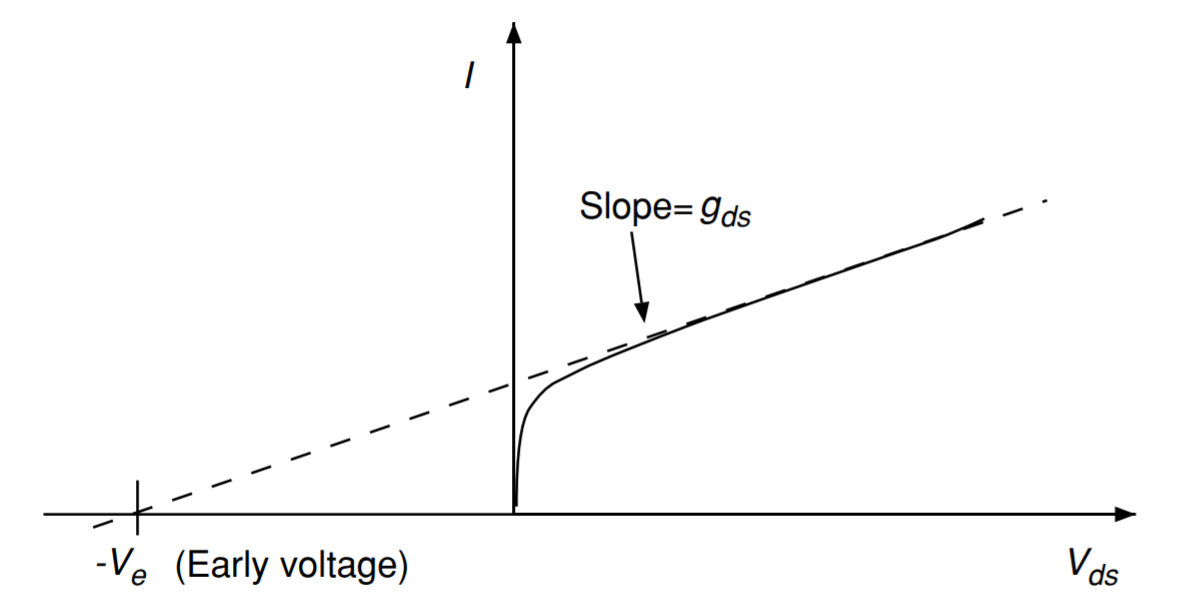
\includegraphics[width=0.95\linewidth]{../../Figures/Early_Voltage.PNG}
    \caption{Plot of current versus drain-to-source voltage, showing the slope of the curve gds in the saturation regime. The intersection of the slope with the Vds axis is called the Early voltage. Adapted from Lecture Notes.}
    \label{fig:basalandcerebellum}
\end{figure}

We just established that even in Saturation, there is a slight increase in $I_{ds}$ as a function of increasing $V_{d}$ - this increase is linear as shown in the figure above, and it has a very specific slope called $g_{ds}$, also called the \emph{output conductance} of the transistor. It is defined as follows: 

\begin{equation}
g_{ds} = \frac{\partial I}{\partial V_{ds}} = \frac{\partial I}{\partial L_{eff}}\frac{\partial L_{eff}}{\partial V_{ds}} = \frac{I}{V_e}
\end{equation}

$V_{e}$ is the \emph{Early Voltage}, which is defined as the \textbf{absolute value of voltage for which $I_{ds}$ is 0} when in saturation. It is only a theoretical voltage that allows you to quantify the steepness of the $I_{ds}$ slope in saturation, and thus the extent by which $I_{ds}$ changes as a function of $V_{ds}$ changes. 
Understanding the precise derivation of the equation requires a substantial amount of device physics, which is out of the scope of these lecture notes. If you would like to understand better, refer to the textbook \cite{liu2002analog}, Chapter 3. Now taking the previous equation as granted, we can rewrite our equation for drain current in a more complete manner, as follows:

\begin{equation}
    I = I_{sat} + g_{ds}V_{ds} = I_{sat}(1 + \frac{V_{ds}}{V_e})
\end{equation}

Here, $I_{sat}$ =  $I_{n0} e^{\frac{\kappa_{n}V_g - V_s}{U_T}}$
Should you really care about this second order effect? Yes, because $V_E$ ranges between 750V and 20V for typical transistors operating in Subthreshold, as shown in the figure below: 

\begin{figure}[H]
    \centering
    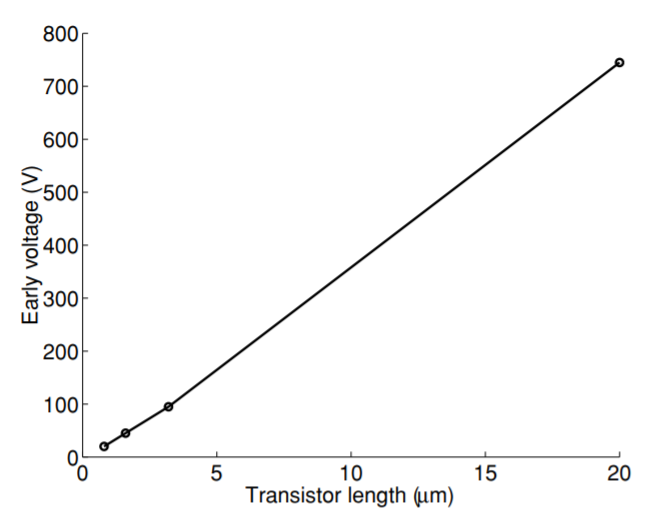
\includegraphics[width=0.95\linewidth]{../../Figures/Early_Voltage_Vs_MOSFET_Length.PNG}
    \caption{Early voltage versus the transistor length of an nFET fabricated in a 0.8 $\mu m$ CMOS proces. Adapted from Lecture Notes.}
    \label{fig:basalandcerebellum}
\end{figure}

Keep in mind that 20V is a way more significant Early Voltage than 750V, because that equates to a lot steeper slope! This is why Early Voltage is particularly important in shorter MOSFETs: a slight change in $V_{ds}$ will have significant impact on $I_{ds}$ when in Saturation! The smaller the transistor, the smaller $V_E$, and the smaller $V_E$, the higher $\frac{\partial I}{\partial V_{ds}}$. 
